\label{chap:p5-tlds}
\section*{Preamble}
During the erythema study (Chapter~\ref{chap:p4-imrt_study}), weekly dose measurements were performed by placing thermoluminscent detectors (TLDs) inside patient masks in the DRS measurement area. This data was used in that paper to interpret patient responses to radiation therapy. Since the measurements were taken every week on every patient, there was the possibility of further analysis on the collected data. TLDs are used for so many purposes across so many disciplines, that their dose response uncertainties are well understood to be around 2-3\%, depending on the calibration procedure. However, this does not address what kind of differences should be expected for repeat measurements in-phantom or \emph{in vivo}. To determine a representative uncertainty, the TLD results were statistically analyzed and a limited investigation into the source of the variation was completed.

Outside of the assistance provided for the previous paper, the majority of the work was performed by the author of this thesis (further known as ``the author''). The TLD measurements were all performed by the author, although they could not have been collected without the cooperation of the radiation therapy teams at the Juravinksi Cancer Centre (JCC). The author was trained in the use of the TLD reader and proper TLD calibration techniques by Ms. L Gamble and was supported in the endeavor by all of the members of the Physics Quality Assurance team at the JCC. The manuscript was prepared in collaboration with Dr. O. Ostapiak and was additionally reviewed by Drs. T. Farrell, J. Hayward, J. Wright, and Mrs. Doerwald-Munoz. The manuscript has been altered from its original form to match the style of this thesis.

\section*{Contents}

\begin{center}
	
	\textbf{Thermoluminescent dosimeter placment uncertainty in intensity-modulated radiation therapy thermoplastic masks}
	
	Diana L. Glennie, Orest Z. Ostapiak, Joseph E. Hayward, Lillian Doerwald-Munoz, James Wright, and Thomas J. Farrell
	
	\textit{Department of Medical Physics and Applied Radiation Sciences, McMaster University, 1280 Main Street West, Hamilton, Ontario, L8S 1A8}
	
	\textit{AND}
	
	\textit{Department of Medical Physics, Juravinski Cancer Centre, 699 Concession Street, Hamilton, Ontario, L8V 5C2}
	
\end{center}

\noindent Submitted to the \textit{Journal of Applied Clinical Medical Physics} on November 5, 2014.

\section{Introduction}
Thermoluminescent dosimeters (TLDs) are commonly used for phantom and \emph{in vivo} dosimetry to confirm radiation therapy dose calculations\cite{Essers1999,Mijnheer2013} and a large amount of research has established the random and systematic uncertainties related to the TLD dose measurement procedure.\cite{Kirby1992,Mijnheer1987} On average, TLDs are expected to have a standard deviation of 2-3\% when properly calibrated.\cite{Essers1999,Ostwald1995} However, this uncertainty is expressed for TLDs irradiated in a uniform treatment field where there is no added uncertainty due to patient or TLD positioning. In the case where TLD measurements must be performed several times during a single patient’s radiation therapy treatment to monitor progress or to confirm the calculated dose, it would be useful to have a measure of the TLD reproducibility that includes possible treatment setup errors and TLD positioning errors. Currently, \emph{in vivo} dosimetry research with TLDs focuses on the difference between the TLD measurements and the calculated dose,\cite{Ruden1976,Leunens1990,Tung2004} not on measurement reproducibility due to patient and TLD positioning uncertainty. This knowledge would allow for the determination as to whether or not separate session measurement differences in the TLD reading from are significant and should be further investigated.

\section{Methods}
Ten patients undergoing radiation therapy for head and neck cancer at the Juravinski Cancer Centre (Hamilton, Ontario, Canada) were enrolled in a prospective, observational study to monitor radiation-induced erythema.\cite{Glennie2014c} The prescribed doses were either 60 or 70 Gy to a reference point within the tumor target, delivered in 2 Gy fractions. All treatments were planned using intensity modulated radiation therapy (IMRT) and required an immobilizing thermoplastic mask. In order to compare the erythema to the received skin dose, TLD measurements were performed weekly throughout treatment.

\subsection{TLD Measurements}
Each week, during the course of treatment, a TLD array was placed inside the patient masks. The TLD array consisted of five packets of two TLDs placed in a cross configuration on a square piece of paper (approximately 7 cm x 7 cm). The group of TLDs were maintained on site, and were batched such that each had a calibrated uncertainty of 2.9\%. The location of the array was selected based on the area of projected maximum skin dose as determined from the radiation therapy plan developed using the Pinnacle3 (Philips, Andover, MA) Radiation Therapy Planning System (TPS).

Following each measured irradiation, the TLDs were read on site with a commercial TLD reader (Harshaw TLD 5500, Saint-Gobain Crystals \& Detectors, Hiram, OH). None of the TLD pairs differed by more than the reading uncertainty (2.9\%), although there were 7 instances where one of the TLDs returned an error during the reading process. Given this low difference between the TLDs in a pair, their average was used as the dose for each TLD packet location. When one of the TLDs returned an error, the single remaining TLD dose was used instead of the average. For each location on the skin, there was a TLD data set of 5-7 measurements collected over the course of treatment.

\subsection{Statistical Analysis}
A descriptive statistical analysis of the results requires that there be no trends in the sets of TLD data, such as time dependence. Time dependence is a valid concern, as weight loss is often observed over the course of treatment of head and neck cancer, which could affect the mask fitting and consequently, the measured dose. To test whether each data set is time independent (i.e., could be a member of a completely uncorrelated parent population), the Pearson correlation coefficients were calculated to test the reciprocity between the TLD dose and week of treatment for each TLD position.\cite{Bevington2003}

The mean and standard deviation for each of the measured TLD dose data sets was calculated. Following a test for a dose dependence of the standard deviations, descriptive statistics were performed on the standard deviations and further dependence tests were performed to determine the source of the variation.

\subsection{TPS Calculated Dose at TLD Location}
Information regarding the calculated dose at the TLD site was determined using the TPS. Following the final radiation fraction, radio-opaque fiducial markers were placed inside each patients’ mask at the exact location of each TLD packet, and the masks were scanned with CT. These scans were registered with the original planning image set. TLD chip packets were represented in the TPS by regions of interest (ROI) with the same dimensions (0.94 cm x 0.44 cm x 0.18 cm). These regions were placed to coincide with the marker positions at three different depths: 1) on the skin surface (“skin surface”), 2) straddling the skin surface (“mid-skin”), and 3) just below the skin surface (“in-skin”). The voxel size was defined by the dose grid dimension of 0.25 cm. As a result, the TLD ROI spanned 6 voxels in the treatment plan. The standard deviation of the average dose across these voxels was recorded for each TLD position.

\subsection{Relationship between the Standard Deviations and TPS Dose Gradients}
To understand the source of the variation in the TLD dose measurements, the standard deviations were compared against their corresponding TPS calculated dose gradients perpendicular and parallel to the skin surface. Since only the relationship between these quantities was investigated, proxy variables were used instead of the exact dose gradients. The dose gradient perpendicular to the skin, referred to here as the depth dose gradient, was approximated by subtracting the skin surface dose from the in-skin dose as follows,

\begin{equation}
	\nabla D_{depth} = D_{in~skin} - D_{surface}	
\end{equation}

The standard deviation within each TLD ROI in the TPS patient plan was used to represent the surface dose gradient in the plane of the skin.

\section{Results}
In total, 50 sets of TLD measurements were collected on ten patients (five sites per patient). For each TLD data set, the interquartile range test was used to identify outliers. Thirty-eight individual TLD measurements were removed (less than one from each location). One data set was removed due to the addition of bolus under the patient mask during the course of treatment.

\subsection{Testing Temporal Independence}
For each TLD data set, the Pearson correlation coefficient was used to determine the probability that there existed a correlation between the measurements and week of treatment. Four of the 49 data sets had p-values less than 0.05, indicating that there was very low probability that they were uncorrelated. These four data sets represent 8\% of the total, only slightly higher than would be expected by chance if they were all completely uncorrelated (5\%). Therefore, it was concluded that there was no significant relationship between the measured TLD dose and time, thus satisfying the requirements for subsequent analysis of the individual TLD sets by descriptive statistics, and the mean and standard deviation of each TLD data set was calculated.

\subsection{TLD Dose Variation}
In order to test the relationship between the standard deviations and their corresponding means, the Pearson correlation coefficient was calculated and no dose dependence was found (p = 0.27).    It is usual to express the uncertainty in a TLD measurement as a percent. However, when the standard deviations were expressed as percentages of the corresponding means, there was a dose dependence that would prevent further statistical analysis (p = 2.3E-04). Therefore all subsequent analysis was performed on the standard deviations and the relative standard deviations were not further analyzed. The mean, median, and first and third quartiles of the standard deviations are shown in Table~\ref{tab:descrip_stats}.

\begin{table}[h]
	\centering
	\caption{Descriptive statistics for the standard deviations from each TLD location.}
	\label{tab:descrip_stats}
	\begin{tabular}{|l|l|}
		\hline
		Mean           & 6.7 cGy  \\ \hline
		Median         & 4.8 cGy  \\ \hline
		First Quartile & 3.0 cGy  \\ \hline
		Third Quartile & 8.6 cGy  \\ \hline
		Range          & 23.8 cGy \\ \hline
	\end{tabular}
\end{table}

Since there is no dose dependence, the standard deviation of each of the data sets can be treated as an independent sample of a greater population and, therefore, can be used to estimate the additional variance due to TLD positioning error. Since they do not follow a normal distribution, the mean of the standard deviations (6.7 cGy) does not represent the population’s standard deviation. According to Cochran’s theorem,\cite{Knight1999} the sample variances should follow a scaled chi-squared distribution. For such a distribution, a better measure of the population variance is the expectation value of the sampled variances, which would be equal to the mean of the square of the sample standard deviations. That is,

\begin{equation}
	\label{eq:cochran}
	\sigma^2 \sim E\left(s^2\right) = \frac{\sum_{i=1}^n \left(s_i^2\right)}{n}
\end{equation}

The TLD sample standard deviations follow this scaled chi-squared distribution, as shown in Figure~\ref{fig:p5-stdev_histogram}. Therefore, the population standard deviation was approximated from these data as 8.7 cGy using Equation~\ref{eq:cochran}.

\begin{figure}
	\centering 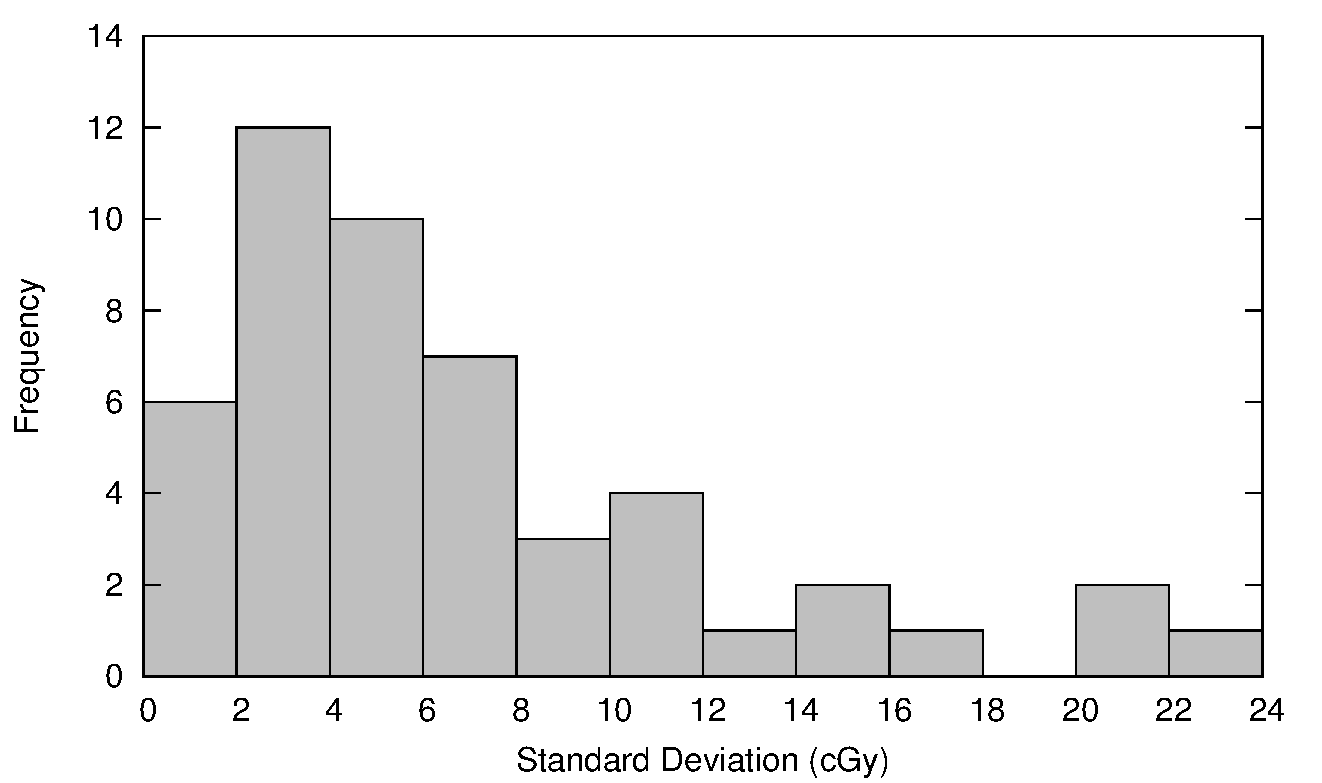
\includegraphics[width=0.6\textwidth]{figures/p5-stdev_histogram.png}
	\caption[A histogram of the standard deviations for the 49 TLD data sets]{\label{fig:p5-stdev_histogram}A histogram of the standard deviations for the 49 TLD data sets.}
\end{figure}

\subsection{Gradient Dose Dependence}
The Pearson correlation coefficient was used to test for a dependence between the sample standard deviations and the corresponding TPS calculated surface and depth dose gradients. No statistically significant relationship was found with any of the three surface dose gradient proxies (p\textsubscript{in-skin} = 0.70, p\textsubscript{skin-surf} = 0.50, p\textsubscript{mid-skin} = 0.47). There was also no relationship found between the sample standard deviations and the depth dose gradient proxy (p = 0.10).

\section{Discussion \& Conclusions}
The TLD dose data sets at each measurement location were shown to be independent of time and therefore the calculation of the standard deviation was considered valid. Forty-nine samples of TLD standard deviation were obtained. Since no dose dependence was found for these sample standard deviations, it was also valid to infer the population standard deviation from these values. The population standard deviation was approximated to be 8.7 cGy from the expectation value of the sample variance. This corresponds to 4.4\% to 74.0\% for the range of doses observed in this study. However, if doses below 83.1 cGy are excluded (by the interquartile range outlier test), the uncertainty does not exceed 10.5\%. Therefore, the TLD reproducibility, including patient and TLD positioning variation, is 10.5\%. This is 7.5\% greater than the inherent uncertainty associated with TLDs irradiated in a uniform field.

No relationship was found between each location’s standard deviation in dose and TPS calculated depth dose gradient. This can be explained by the fact that the TLD is always positioned on the skin surface. Any motion of the TLD along the depth dose gradient direction would involve movement of the skin surface and a corresponding movement of the depth dose gradient. Similarly, no relationship was found between each location’s standard deviation in dose and the surface dose gradient surrogate. This suggests that a single dose calculation in the TPS does not adequately represent the variation in dose within the TLD due to patient setup error. Further investigation would require simulating patient setup error within the TPS through successive displacements of the isocenter.

Aside for the TLD placement and patient positioning uncertainties, it is possible that some of the measured dose variation was due to the mask perforation pattern. As established by Lee et al.\cite{Lee2002}, thermoplastic immobilization masks have measurable shielding and build-up effects. This has the potential to contribute to the measured dose variation if the TLDs are positioned near a gap in the mask plastic.

This study investigated the reproducibility of TLD measurements in a clinical setting. The TLD measurement uncertainty was found to be three times larger (10.5\%) than the standard calibration uncertainty for TLDs in a uniformly irradiated field. When performing in vivo dosimetry, it is common practice to report and investigate the dose discrepancy when the difference between the measured and planned doses exceeds 5\%.\cite{Essers1999} However, this study suggests that some of these discrepancies could be attributed to TLD and patient positioning errors that have not been accounted for. The results of this study could be strengthened by an expanded sample size with additional measurements. Instead of weekly measurements that resulted in 5-7 TLD readings, dose measurements could be performed daily, resulting in up to 35 individual samples for each measurement location.

\section*{Acknowledgments}
This work was financially supported by the Natural Sciences and Engineering Research Council of Canada.